% Lesson: my radio, from the terminal player on the Macs to the buffered iPhone page on AlfDROID.
% Compile with:  latexmk  (settings in .latexmkrc)

\documentclass[11pt,a4paper]{article}

\usepackage{fontspec}
\usepackage[margin=2.2cm]{geometry}
\usepackage{xcolor}
\usepackage[most]{tcolorbox}
\usepackage{listings}
\usepackage{twemojis}
\usepackage{alfdoc}
\usepackage[inline]{enumitem}
\usepackage{booktabs}
\usepackage{array}
\usepackage{graphicx}
\usepackage{tikz}
\usetikzlibrary{positioning,calc,fit}
\usepackage{xurl}
\usepackage[colorlinks=true,linkcolor=blue,urlcolor=blue]{hyperref}
\usepackage[nameinlink,capitalise]{cleveref}

\setlength{\parindent}{0pt}
\setlength{\parskip}{0.6em}
\setlength{\emergencystretch}{3em}

% Review round open for revision 2: the Boox notes arrived on the 16 Nov PDF (revision 1).
\reviewtrue

\title{\emo{radio}\ \name{Radio}\\[0.3em]
  \large Eight stations in the Mac's terminal, and on \name{AlfPHONE} three minutes behind live}
\author{Lesson for Alf, written by Claude}
\date{Sat 14 Nov 2026}

\begin{document}
\maketitle

\section*{What it is}

I listen to eight classical and jazz stations in two places. % Review: ``AlfPHONE''
On the Macs, \name{radio} plays them in a terminal pane through \name{mpv}, a command-line media player, with each station's name in large block letters and a line for every piece. \here[AlfPHONE throughout][Every ``the iPhone'' that means my phone becomes \name{AlfPHONE}; the model name iPhone 13 and the phone's screen width stay as they are.] On \name{AlfPHONE}, a web page served by \name{AlfDROID}, the OnePlus 6 that runs as a server at home, plays them through Safari. The phone listens three minutes behind the live broadcast, so it holds three minutes of music in its own memory, and a subway ride between stations, where the train loses the network for a minute or two, plays through without a break.

% Review: ``I think this needs capitalization similar to iPhone and Macs''
Everything lives in one folder, \name{\textasciitilde/.settings/Scripts/radio}, in my settings repo, cloned on both Macs and on \name{AlfDROID}: \here[AlfDROID throughout][The machine's name is \name{AlfDROID} everywhere, possessives included, replacing ``the droid''.]

\begin{itemize}[nosep]
  \item \textbf{\name{radio.m3u}}: the eight stations and their stream addresses.
  % Review: ``why the underscore if all the other names use the dash''
  \item \textbf{\name{radio\_core.py}}: the rules both players share for the titles the stations send. \here[underscore, not dash][Python imports the file as a module, and a module name cannot carry a dash.] The name has an underscore because Python imports it as a module, and a dash cannot appear in a module name.
  \item \textbf{\name{mpv.conf}} and \textbf{\name{radio.lua}}: the terminal player, an \name{mpv} profile and its script.
  \item \textbf{\name{radio}}: the command on the Macs. Alone it plays; its subcommands look after \name{AlfDROID}.
  \item \textbf{\name{radio-server.py}}: the service on \name{AlfDROID}, with the relays, the tapes, the covers, and the page and its streams.
  \item \textbf{\name{radio-page.html}}: the page \name{AlfPHONE} opens.
  \item \textbf{\name{logos-dark}}: draws dark versions of the bright station logos.
  % Review: ``we will change this name because it's inside of alfdroid so it's a component it's not a standalone thing''
  \item \textbf{\name{install.sh}} and \textbf{\name{boot/radio}}: the installer for each machine, and \name{AlfDROID's} start at boot, which also starts \here[AlfDROID's Funnel][It is a second \name{Tailscale} inside \name{AlfDROID}, a component of the machine and not a standalone device, so it is named \name{AlfDROID's Funnel}.] \name{AlfDROID's Funnel}, \name{AlfDROID's} public address.
\end{itemize}

\Cref{fig:parts} shows how the pieces sit on the three machines. The Mac plays the stations straight from the internet. \name{AlfDROID} also takes them from the internet, keeps the last five minutes of each in memory, and serves them to \name{AlfPHONE} in two ways: over the tailnet, my private network between my devices, and through a public address on the internet, which works when the phone's tailnet does not.

\begin{figure}[ht]
\centering
\begin{tikzpicture}[font=\small,
  box/.style={draw, thick, rounded corners=3pt, align=center, inner sep=4pt},
  host/.style={draw, thin, rounded corners=6pt, inner sep=6pt, draw opacity=.35},
  lab/.style={font=\scriptsize, align=center}]
  % Positions on a grid, so no box crosses another
  \node[box, draw=grey!80!black] (st) at (0.25,3) {8 stations\\ \scriptsize MP3 and AAC streams};
  \node[box, draw=orange] (ff) at (5.2,3) {\name{ffmpeg}, one per station\\ \scriptsize re-encodes to 128 kbit/s MP3};
  \node[box, draw=green] (ice) at (3.6,1.5) {\name{icecast}\\ \scriptsize :8001, live};
  \node[box, draw=blue] (tape) at (6.8,1.5) {tapes in RAM\\ \scriptsize 5 min per station};
  \node[box, draw=aqua] (srv) at (6.8,0) {\name{radio-server.py}\\ \scriptsize :8080, page, HLS, status};
  \node[box, draw=pink] (ar) at (9.6,3) {\name{AlfDROID's Funnel}\\ \scriptsize second Tailscale, :8443};
  \node[host, fit=(ff)(ice)(tape)(srv)(ar), label={[lab]above:\name{AlfDROID}: OnePlus 6, \name{Termux}}] {};
  \node[box, draw=grey!80!black] (rel) at (13.5,3) {Funnel relay\\ \scriptsize Tailscale's servers};
  \node[box, draw=red] (ph) at (13.5,0) {Safari\\ \scriptsize the page, HLS};
  \node[host, fit=(ph), label={[lab]below:\name{AlfPHONE}: iPhone 13}] {};
  \node[box, draw=lavender] (mpv) at (0.25,-2) {\name{mpv} and \name{radio.lua}\\ \scriptsize with \name{radio\_core.py}};
  \node[box, draw=violet] (cmd) at (6.8,-2) {the \name{radio} command\\ \scriptsize status, watch, on, off, \ldots};
  \node[host, fit=(mpv)(cmd), label={[lab]below:a Mac}] {};
  \draw[->] (st) -- (ff);
  \draw[->] (st) -- node[lab, left] {internet} (mpv);
  \draw[->] (ff) -- (ice);
  \draw[->] (ff) -- (tape);
  \draw[->] (tape) -- (srv);
  \draw[->] (srv.north east) -- (ar.south);
  \draw[->] (ar) -- node[lab, above] {tailnet} (rel);
  \draw[->] (rel) -- node[lab, right] {internet} (ph);
  \draw[->] (srv) -- node[lab, above, pos=0.62] {tailnet} (ph);
  \draw[->] (cmd) -- node[lab, right] {tailnet: API and \name{ssh}} (srv);
\end{tikzpicture}
\caption{The parts and the machines they run on. Arrows follow the audio, except the \name{radio} command's, which follow its requests. The phone reaches the page in two ways: over the tailnet, or from the internet through \name{AlfDROID's Funnel}, a second \name{Tailscale} on \name{AlfDROID} whose Funnel takes requests from Tailscale's relay.}
\label{fig:parts}
\end{figure}

\section*{Stations and their titles}

\name{radio.m3u} lists the stations in the order the players number them: Classic FM, Radio Swiss Classic, Venice Classic Radio, WQXR, Rai Radio Classica, Radio Swiss Jazz, Jazz24, and Secret Agent. Each line holds a stream address, an endless MP3 or AAC file that the station's server keeps sending.

% Review: ``there are three names and I don't know any of these''
A station names the piece it is playing inside the stream itself, with a scheme called icy metadata. \here[what these are][SHOUTcast and Icecast are the two programs that run a station's server, and icy metadata is their scheme for putting the playing piece's title into the stream.] The scheme comes from \name{SHOUTcast} and \name{Icecast}, the two programs that commonly run a radio station's server and send its stream to listeners, and it is how they put the title of the playing piece into the stream~\cite{icy}. A player that sends the header \texttt{Icy-MetaData: 1} gets a reply header \texttt{icy-metaint}, a byte count. After every that many bytes of audio, the station inserts one byte, a length in units of 16 bytes, then a text block of that length, such as \texttt{StreamTitle='Johannes Brahms - Hungarian Dances';}. A length of zero means no new text.

% Review: ``1,2,3''
The titles arrive in rough shape, and \name{radio\_core.py} holds the three rules both players apply to them, so the Mac and \name{AlfDROID} agree on what a piece is:
\begin{enumerate}[nosep]
  \item \here[numbers 1, 2, 3][The three rules are now an enumerate, so they carry the numbers 1, 2, and 3.] Some stations encode their accents twice, so \texttt{é} arrives as \texttt{é}, and the rule undoes that.
  \item A station announces itself between pieces and sends the announcement as the title, so the rule drops a title that is only the station's own name.
  \item A player hears the same title many times while a piece plays, so the rule writes each piece to the log once.
\end{enumerate}
\texttt{radio\_core.py -{}-selftest} checks these rules against titles the stations really sent, and runs at the end of every install.

\subsection*{Rai's pieces}

One station carries its titles outside the stream. Rai Radio Classica announces \texttt{icy-metaint: 16000} and then fills every block with an empty title. A listener left on its stream for 30 minutes on Sat 14 Nov received 414 blocks, every one of them \texttt{StreamTitle='';}.
% Review: ``is this another bug did I forget to add the title should I use zero metadata in case they are actively sending nothing''
\here[Rai's own behaviour][These empty blocks are the station's own behaviour: each one carries an empty title.] The empty titles are the station's own behaviour: every block of its stream carries \texttt{StreamTitle='';}. Rai's public schedule, \url{https://www.raiplaysound.it/palinsesto/onAir.json}, names only the running programme, such as \textit{Classico notturno}. Rai's own player shows the piece, because it asks a second Rai service for it, and \name{AlfDROID} asks that service the same way, in three steps, as \cref{fig:rai} shows.

\begin{enumerate}[nosep]
  % Review: ``why there is an expiration here''
  \item \textbf{A token.} \name{AlfDROID} asks \url{https://www.raiplaysound.it/atomatic/token-service/api/jwt-ws} for a token, with a client id made from the page's address. The answer is a signed JSON Web Token that expires after an hour, together with the server to connect to and the prefix of its topics. \here[token carries expiry][A signed token carries its own expiry time, so a stolen one stops working on its own.] The token carries its expiry time inside its signature, so a stolen one stops working on its own.
  % Review: ``same as before this is a little too hard for me to understand''
  \item \textbf{A connection.} \here[easier two sentences][The MQTT and WebSocket sentence became two short sentences, each term explained where it first appears.] \name{AlfDROID} connects to \name{prod.rai.harperfabric.com} over a WebSocket, a two-way connection that stays open over HTTPS so either side can send at any moment. Messages travel on it with MQTT, a lightweight protocol in which the server pushes each new message to the listener as it happens. The token goes in the address, after \texttt{/mqtt?jwt=}.
  \item \textbf{A subscription.} \name{AlfDROID} subscribes to the channel's topic, the name under which the server sorts its messages, here \texttt{ws/rai-radio-3-classica}. The server keeps the newest message of every topic and hands it over at once, so the piece playing now arrives first, and one more message arrives at each change of piece.
\end{enumerate}

Each message is JSON. Its \texttt{now} object holds the piece in capitals in \texttt{caption}, such as \texttt{BEETHOVEN LUDWIG VAN QUARTETTO IN FA MIN OP. 95\ldots}, and the moment the piece ends in \texttt{expireAt}.

\name{radio-server.py} keeps that subscription open in one thread, with the \name{paho-mqtt} library, and asks for a fresh token before the old one expires. Every caption goes through \texttt{caption\_case} in \name{radio\_core.py}, which turns the capitals into normal case, and then into the same path as any station's title: the page, the queue, and \name{log.tsv}. Between two captions the page shows the programme from the schedule, which stays out of the log. \name{AlfDROID} is the only machine that talks to Rai, and the terminal player gets Rai's title from \name{AlfDROID's} \texttt{/api/status}.

\begin{figure}[ht]
\centering
\begin{tikzpicture}[font=\small, y=0.75cm,
  box/.style={draw, thick, rounded corners=3pt, align=center, inner sep=4pt, minimum width=3.4cm},
  lab/.style={font=\scriptsize, above}]
  % One lifeline per party; time runs downwards
  \node[box, draw=aqua] (d) at (0,0) {\name{radio-server.py}\\ \scriptsize on \name{AlfDROID}};
  \node[box, draw=orange] (t) at (5,0) {token service\\ \scriptsize \name{raiplaysound.it}};
  \node[box, draw=red] (m) at (10,0) {MQTT server\\ \scriptsize \name{prod.rai.harperfabric.com}};
  \foreach \x/\n in {0/d,5/t,10/m} \draw[draw opacity=.35] (\n.south) -- (\x,-7.4);
  \draw[->] (0,-1.5) -- node[lab] {1. a token, for this client id} (5,-1.5);
  \draw[->] (5,-2.4) -- node[lab] {token, server, topic prefix} (0,-2.4);
  \draw[->] (0,-3.4) -- node[lab, pos=0.75] {2. connect with the token} (10,-3.4);
  \draw[->] (0,-4.4) -- node[lab, pos=0.75] {3. subscribe to the topic} (10,-4.4);
  \draw[->] (10,-5.4) -- node[lab, pos=0.25] {the current caption, at once} (0,-5.4);
  \draw[->] (10,-6.4) -- node[lab, pos=0.25] {a new caption at each piece} (0,-6.4);
\end{tikzpicture}
\caption{How \name{AlfDROID} gets Rai's pieces, with time running downwards: a token from Rai's token service, then a connection and a subscription on Rai's MQTT server, which sends the current caption at once and a new one at each change of piece.}
\label{fig:rai}
\end{figure}

\section*{In the terminal}

On a Mac, \texttt{radio} alone starts \name{mpv} with the \texttt{radio} profile from \name{mpv.conf}. The profile loops the playlist, hides \name{mpv}'s own messages, and loads \name{radio.lua}, the script that draws the pane. For each station, the script prints its name in block letters, in a colour of its own from the ColorBrewer Set3 palette, with the stream's format, bitrate, sample rate, and channels underneath. It then prints a line for each new piece, with the time it started.

\begin{cmdout}
5/8  ·  mp3  ·  256 kbps  ·  44.1 kHz  ·  stereo  ·  coreaudio
\end{cmdout}

The keys are \texttt{1}--\texttt{8} and letters to jump to a station, \texttt{<} and \texttt{>} to step, \texttt{9} and \texttt{0} for the volume, \texttt{c} for a menu of what every station is playing now, \texttt{space} to pause, \texttt{l} to like the piece that is playing, and \texttt{q} to quit. The status line at the bottom shows the piece, the time, and the volume, and it says \texttt{paused} in orange while the player is paused, because a paused station otherwise looks like a dead one stuck at 00:00:00.

A piece that has played for 30 seconds on one station goes into \name{\textasciitilde/.local/share/radio/log.tsv} as date, time, station, and piece. The 30 seconds keep out the pieces I skipped past. \name{AlfDROID} writes its own \name{log.tsv} in the same shape, so each machine keeps its own listening history.

The \texttt{l} key keeps a piece I want to hear again. The player asks \name{AlfDROID's} \texttt{/api/like} with the station and the piece, and \name{AlfDROID} adds the piece to \name{liked.json}, or removes it when it is already there. The player answers with a short message, \texttt{liked} or \texttt{unliked}, led by a filled or an empty heart. \name{liked.json} lives only on \name{AlfDROID}, so the page and every terminal share one list. Each entry holds the time, the station's slug and name, and the piece.

\section*{\name{AlfDROID's} service}

\texttt{./install.sh droid} installs \name{ffmpeg}, \name{icecast}, and Python with \name{Termux}'s package manager and puts \name{radio-server.py} on \name{AlfDROID's} \texttt{PATH}; \texttt{-{}-boot} also installs \name{boot/radio}, which \name{Termux:Boot} runs when the phone starts, so the service comes back by itself after a reboot. \texttt{./install.sh mac} links the player's files into \name{mpv}'s config folder and \name{radio} into \name{\textasciitilde/.local/bin}.

\name{radio-server.py} runs one \name{ffmpeg} per station. Each \name{ffmpeg} reads the station's stream and re-encodes it to 128 kbit/s MP3, so all eight streams come out in one format whatever the station sends: Rai, for one, sends 256 kbit/s. \name{ffmpeg}'s \texttt{tee} output sends the result to two places at once: to the local \name{icecast} on port 8001, where any player on the tailnet can listen live, and to the server itself, which keeps it on a tape. A supervisor restarts an \name{ffmpeg} that stops, with a growing pause between attempts. Further threads follow each station's titles, write the log, and fetch the station logos once.

The recording switch starts and stops every relay together, and a station can be muted on its own. \texttt{radio record} records every station to tape and \texttt{radio stop} stops them all; with station names, both act on those stations only, so \texttt{radio record jazz24} with the recording off records Jazz24 alone. Both are saved to \name{muted.json}, so a restart keeps them. An idle watchdog switches recording off after 15 minutes with no listener, so an evening I forget to switch it off costs \name{AlfDROID} nothing. The watchdog starts its clock when the service starts.

On \name{AlfDROID} the relays take a measurable share of the phone. One reading of \texttt{top} on Sat 14 Nov showed each \name{ffmpeg} at 16--32\% of one core and the server at 8\%, on a phone with eight cores.

\section*{Tape and buffer}

The \emph{tape} is \name{AlfDROID's} recording of one station: the last 300 seconds of its re-encoded audio, held in RAM and refilled as the station plays. It lives in memory because the phone's flash storage wears out with constant writing, and a restart of the service empties every tape. The \emph{buffer} is the audio \name{AlfPHONE} has already downloaded and not yet played. The page listens 180 seconds behind live, so a full buffer holds three minutes: everything from the playhead up to the live edge.

The tape is measured in bytes. A 128 kbit/s MP3 carries 128k bits each second, which is 16k bytes:

\[ \frac{128\,000\ \text{bit/s}}{8\ \text{bit/byte}} = 16\,000 \tag*{[byte/s]} \]

So a request for three minutes behind live starts this many bytes before the end of the tape:

\[ 180\ \text{s} \times 16\,000\ \text{byte/s} = 2\,880\,000 \tag*{[byte]} \]

The constant matters. With 16\,384 bytes per second, which is 128 times 1024, the same request reached 2\,949\,120 bytes back, 184 seconds of audio, and the phone showed a buffer of 3:04.

\Cref{fig:tape} shows the two together. The tape spans five minutes up to the live edge. The playhead sits three minutes back, and the buffer is the stretch from the playhead to live. When the network drops, the music keeps playing out of the buffer, which shrinks while the playhead and the live edge move on together. When the network returns, the phone downloads the missing stretch from the tape and the buffer is full again. A dropout longer than the buffer runs it dry: the music stops, the playhead stays where it was, and the phone resumes from that spot when the network comes back, later than three minutes behind, as long as that spot is still on the tape.

\begin{figure}[ht]
\centering
\begin{tikzpicture}[font=\small, x=2.4cm, y=1cm]
  % Scale: minutes behind live
  \foreach \m/\l in {-5/{$-5$ min},-4/{$-4$},-3/{$-3$},-2/{$-2$},-1/{$-1$},0/{now}}
    \node[font=\scriptsize] at (\m,3.35) {\l};
  % A faint line down from each minute, through all three rows
  \foreach \m in {-5,...,0} \draw[draw opacity=.15, very thin] (\m,3.15) -- (\m,-0.85);
  % Row 1: playing normally
  \node[anchor=east, font=\scriptsize, align=right] at (-5.15,2.6) {playing};
  \draw[thick, draw=blue] (-5,2.4) rectangle (0,2.8);
  \fill[aqua] (-3,2.43) rectangle (0,2.77);
  \draw[very thick] (-3,2.3) -- (-3,2.9);
  \node[font=\scriptsize] at (-4,2.1) {already heard};
  \node[font=\scriptsize] at (-1.5,2.1) {buffer, 3:00};
  % Row 2: after 1:50 offline
  \node[anchor=east, font=\scriptsize, align=right] at (-5.15,1.2) {1:50 offline};
  \draw[thick, draw=blue] (-5,1.0) rectangle (0,1.4);
  \fill[aqua] (-3,1.03) rectangle (-1.833,1.37);
  \draw[very thick] (-3,0.9) -- (-3,1.5);
  \node[font=\scriptsize] at (-2.42,0.7) {buffer left, 1:10};
  \node[font=\scriptsize] at (-0.92,0.7) {missed, on the tape};
  \draw[->] (-0.92,0.85) -- (-0.92,1.0);
  % Row 3: back online
  \node[anchor=east, font=\scriptsize, align=right] at (-5.15,-0.2) {back online};
  \draw[thick, draw=blue] (-5,-0.4) rectangle (0,0);
  \fill[aqua] (-3,-0.37) rectangle (-1.833,-0.03);
  \fill[green] (-1.833,-0.37) rectangle (0,-0.03);
  \draw[very thick] (-3,-0.5) -- (-3,0.1);
  \node[font=\scriptsize] at (-0.92,-0.7) {refilled in 3 s};
\end{tikzpicture}
\caption{One station's tape (the blue outline) with the playhead (the black mark) three minutes behind live, the buffer (filled), and what a dropout of 1:50 does to it. The tape runs on with the live edge, so the playhead stays at $-3$.}
\label{fig:tape}
\end{figure}

\section*{Getting the buffer onto \name{AlfPHONE}}

A web page plays audio either through Safari's own media player, which takes an address and fetches it by itself, or through MediaSource, a browser interface with which the page fetches the bytes and hands them to the player, so the page decides how much to hold. Chrome on the Mac has MediaSource and the page uses it there. Safari on the iPhone has no MediaSource for MP3, so on the phone the page has to give an address to Safari's player and let the player do the fetching.

The first design gave Safari's player one endless stream that started three minutes back on the tape. \name{AlfDROID's} request log showed what Safari made of it. Safari opened two or three connections for every play: one from the page, one asking for only the first two bytes (\texttt{Range: bytes=0-1}), to probe the file, and the real one. It pulled the whole three minutes, 2.9 MB, in about one second, then kept only part of it. With the page reporting Safari's own count of buffered audio every three seconds, Safari held 48 seconds ahead, steady over four minutes of play, and never more than 64. The player decides that for itself, and the page cannot change it.

HLS, Apple's HTTP Live Streaming~\cite{hls}, is the format Safari's player is built for. The server cuts the stream into short files, the segments, and publishes a playlist that lists them in order. The player downloads the playlist, fetches the segments one after another, and fetches the playlist again to find new ones. On \name{AlfPHONE}, Safari buffered the full three minutes from such a playlist, as the next section shows, so the phone plays HLS.

\subsection*{Segments and the playlist}

\name{AlfDROID} cuts each tape into segments of six seconds. A segment has to start on an MP3 frame, the smallest unit a decoder can play: a 128 kbit/s frame at 44.1 kHz is 417 or 418 bytes long and holds 1152 samples, 26 ms of sound. The server reads each frame's four-byte header as the bytes arrive, and closes a segment once its frames add up to six seconds. A relay that restarts begins a new MP3 stream in the middle of the tape, so the server skips anything that is not a frame and starts a fresh segment there.

HLS requires an audio-only segment to begin with a timestamp~\cite[§3.4 \textit{Packed Audio}]{hls}, so the player can line the segments up: an ID3 tag, the same kind of tag that carries an MP3 file's artist and title, holding a private field named \texttt{com.apple.streaming.transportStreamTimestamp}, a count of 90\,kHz ticks. The server writes that tag in front of each segment's frames as it serves it.

The playlist covers the whole tape, so Safari can buffer from the playhead to live, and tells Safari where to start with \texttt{EXT-X-START}~\cite[§4.3.5.2 \textit{EXT-X-START}]{hls}. Its head on \name{AlfDROID}, with the segments that follow:

\begin{pane}
$ curl -s localhost:8080/classic-fm.m3u8 | head -n 8   # the playlist for Classic FM
\end{pane}
\begin{cmdout}
#EXTM3U
#EXT-X-VERSION:6
#EXT-X-TARGETDURATION:6
#EXT-X-MEDIA-SEQUENCE:0
#EXT-X-START:TIME-OFFSET=-180.0,PRECISE=YES
#EXT-X-PROGRAM-DATE-TIME:2026-11-15T01:43:41.929Z
#EXTINF:6.008,
/hls/classic-fm/0.mp3
\end{cmdout}

\texttt{TIME-OFFSET=-180} asks for a start 180 seconds before the end of the playlist. Each segment carries the wall-clock time it was recorded, \texttt{EXT-X-PROGRAM-DATE-TIME}, from which the page works out how far behind live the playhead is. Safari ignores a start offset that reaches further back than the playlist does and starts near live instead, which happened right after a restart, when the tape held only 96 seconds. The page therefore never asks for more than the tape holds.

\begin{figure}[ht]
\centering
\begin{tikzpicture}[font=\scriptsize, x=0.32cm, y=1cm]
  \foreach \i in {0,...,19} \draw[draw=grey!70!black] (\i,0) rectangle (\i+1,0.6);
  \foreach \i in {20,...,49} \draw[draw=blue, thick] (\i,0) rectangle (\i+1,0.6);
  \foreach \i in {0,10,20,30,40,49} \node at (\i+0.5,-0.25) {\i};
  \draw[very thick] (20,-0.15) -- (20,0.75);
  \node[above] at (20,0.75) {\texttt{EXT-X-START}, $-3$ min};
  \node[above] at (50,0.75) {live};
  \draw[<->] (20,1.25) -- node[above] {fetched at once: the buffer} (50,1.25);
  \draw[<->] (0,1.25) -- node[above] {on the tape, not fetched} (20,1.25);
\end{tikzpicture}
\caption{The playlist over a full tape: 50 segments of six seconds. Safari starts 30 segments, three minutes, before live, fetches all of them at once, then one more every six seconds.}
\label{fig:hls}
\end{figure}

\subsection*{What the phone did}

The page reports Safari's own buffered range to \name{AlfDROID} every three seconds, and \name{AlfDROID} logs every playlist and segment request, so the request log shows exactly what the phone did. On Sat 14 Nov, Radio Swiss Jazz was tapped at 20:46:55 and Safari fetched every segment up to live, reporting 175 to 179 seconds buffered. Airplane mode then went on at 20:48:04 with 178.5 seconds buffered. The music played on from the buffer. At 20:49:54, 1:50 later, the network was back:

\begin{cmdout}
20:49:54 /radio-swiss-jazz.m3u8
20:49:54 /hls/radio-swiss-jazz/44.mp3
20:49:54 /hls/radio-swiss-jazz/45.mp3
|~...~|
20:49:57 /hls/radio-swiss-jazz/62.mp3
20:49:58 /api/status t=192.4 b=185.6
\end{cmdout}

In three seconds Safari fetched segments 44 to 62, 19 segments or 114 seconds of audio, and reported 185.6 seconds buffered again. A plain stream would have given the phone 48 seconds to ride out the same gap.

\section*{The page}

\name{radio-server.py} reads \name{radio-page.html} from disk on every request, so a change to the page reaches the phone on the next reload, with no restart and with the tapes untouched. The page is laid out for the 390-point-wide screen of an iPhone 13, in a dark theme.

\Cref{fig:page} shows the page on the iPhone's width, playing Radio Swiss Jazz, in normal mode and in debug mode. The bar at the top carries the title, \name{AlfDROID radio}, which also switches debug mode on and off, and the REC switch, which starts and stops the recording without playing anything. It shows a red \texttt{● REC} while the tapes are filling and a grey \texttt{○ REC} while they are off. Tapping it at home, a few minutes before leaving, gives the first station tapped on the way a full three-minute buffer at once, because its tape has been filling all along. Under it sit the station picker, with the station's logo and name, a play or pause button, a stop button, and a heart. The heart is grey and empty until I tap it while a piece is playing, and then it turns red and full, and shows that way whenever that piece is the one at the playhead. Under those, the artist and the title of the piece being heard take a line each, and the gauge shows the buffer: a bar in the station's colour and the time it holds, such as 2:59, which turns orange below one minute. A state that needs attention, such as \texttt{connecting…}, \texttt{offline}, or \texttt{paused}, appears in orange at the top right while it lasts, so the gauge keeps its width.

Pause and stop do different things. Pause holds the spot: the music halts, the stream stays open, and play carries on from the same place, so a pause moves the playhead further behind live. Stop closes the stream, and the next play starts fresh, three minutes behind. The lock screen and the AirPods send pause and play, which go to the same two actions.

Debug mode shows the tape for the current station, with a mark for each minute from $-5$ to now, the white playhead, the part already heard, and the part on the phone, and under it \name{AlfDROID's} and the phone's numbers: the download rate, the bytes since the tap, Safari's buffer, and the HLS segment. Under them it shows what \texttt{radio watch} shows in the terminal: each station's relay, tape, and piece, the listeners, and the latest events, newest first, in the stations' colours. \name{AlfDROID} produces that text with the same code as the \name{radio} command, at \texttt{/api/watch}, and the page refreshes it every five seconds and lets it scroll sideways, as a terminal would. At the bottom, debug mode adds three buttons: \texttt{⇣ refill}, which throws away what the phone holds and starts again three minutes behind live with a fresh buffer; \texttt{page}, which loads the page again; and debug off.

The station logos sit on dark tiles, and several are drawn for light backgrounds. \name{logos-dark} fetches the bright ones from \name{AlfDROID}, draws dark versions, and copies them back as \name{\textless slug\textgreater-dark.img}, which the page asks for by name: the two Swiss logos get a black ground with strokes in their own colour, Jazz24 its letters in its own gradient, Secret Agent its red ground sunk to near black, and Rai its white letters without the green box.

\begin{figure}[ht]
\centering
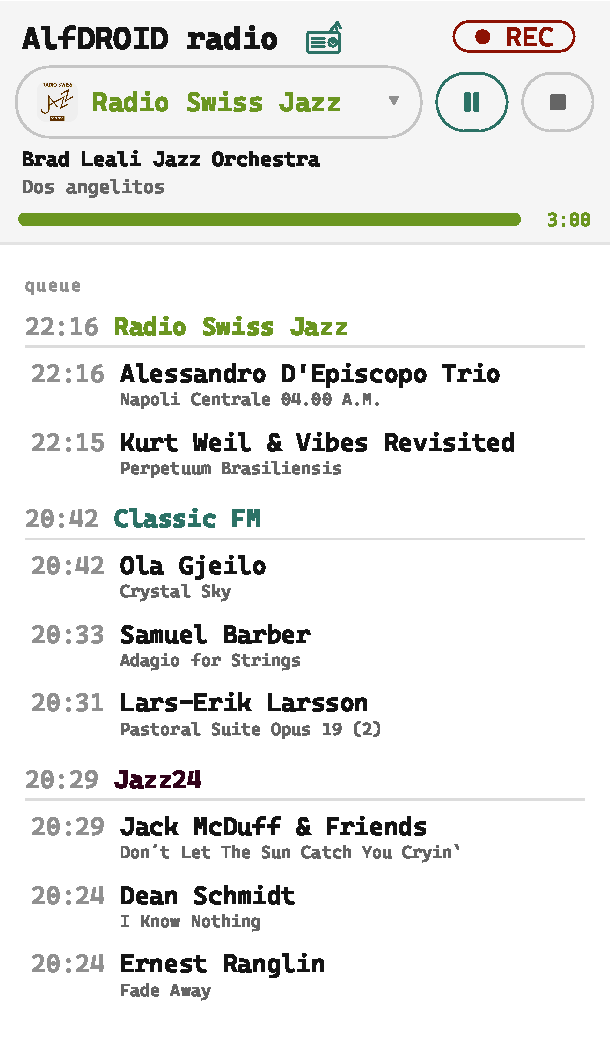
\includegraphics[width=0.42\textwidth]{page.pdf}\hspace{1.5em}%
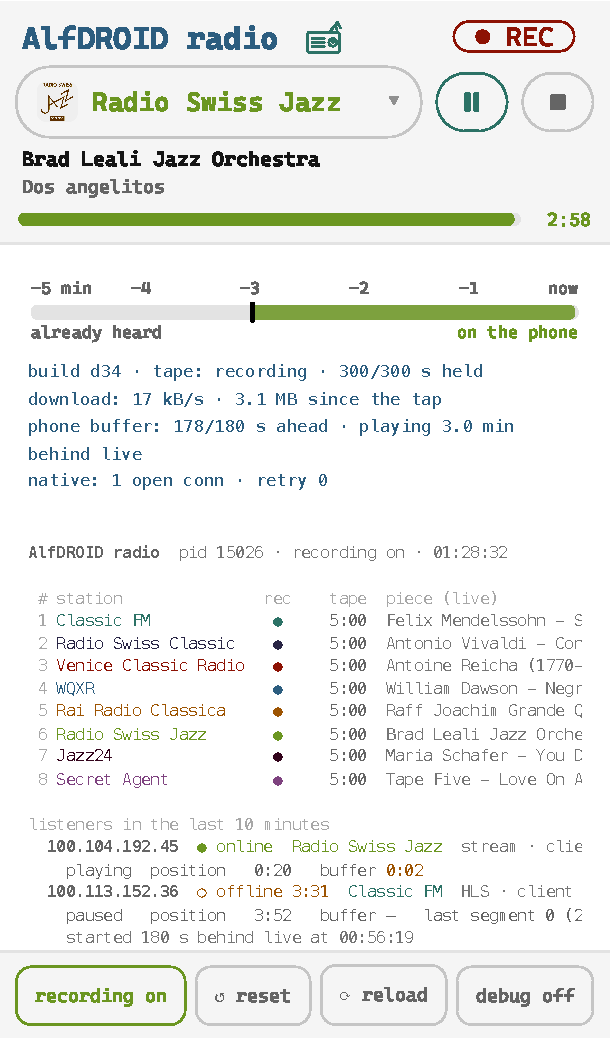
\includegraphics[width=0.42\textwidth]{page-debug.pdf}
\caption{The page at the 390-point width of an iPhone 13, printed from Chrome on the Mac while it played, with each colour's lightness inverted for paper. Left, normal mode: the title and the REC switch, the station, the piece being heard on two lines, the gauge, and the queue of pieces heard. Right, debug mode: the labelled tape, \name{AlfDROID's} and the browser's numbers, the \texttt{radio watch} view, and the debug buttons. Chrome streams the tape directly, so its numbers count connections; on \name{AlfPHONE} that line names the HLS segment.}
\label{fig:page}
\end{figure}

\section*{The piece being heard, and its cover}

A station sends the title of the piece it plays live, and the phone plays that piece three minutes later, so the live title runs three minutes ahead of the music. The server therefore keeps each station's titles with the time they arrived, the page tells the server where it is listening, and the server answers with the piece playing at that moment and a cover for it, as \cref{fig:heard} shows. The page shows that piece, and the log counts it.

\begin{figure}[ht]
\centering
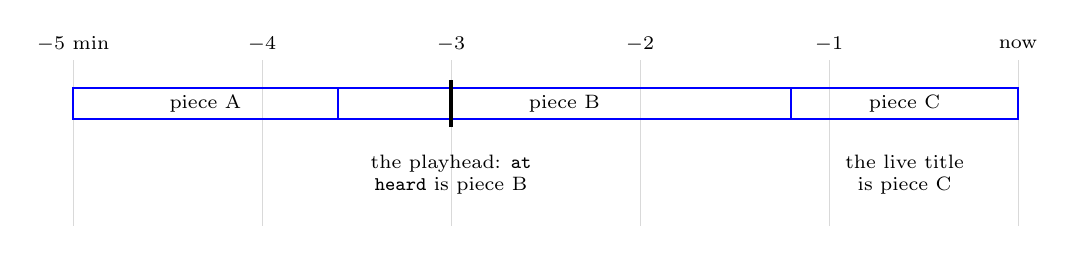
\begin{tikzpicture}[font=\small, x=2.4cm, y=1cm]
  % Scale: minutes behind live
  \foreach \m/\l in {-5/{$-5$ min},-4/{$-4$},-3/{$-3$},-2/{$-2$},-1/{$-1$},0/{now}}
    \node[font=\scriptsize] at (\m,1.35) {\l};
  \foreach \m in {-5,...,0} \draw[draw opacity=.15, very thin] (\m,1.15) -- (\m,-0.95);
  % The tape, cut into the pieces the history names
  \draw[thick, draw=blue] (-5,0.4) rectangle (0,0.8);
  \draw[thick, draw=blue] (-3.6,0.4) -- (-3.6,0.8);
  \draw[thick, draw=blue] (-1.2,0.4) -- (-1.2,0.8);
  \node[font=\scriptsize] at (-4.3,0.6) {piece A};
  \node[font=\scriptsize] at (-2.4,0.6) {piece B};
  \node[font=\scriptsize] at (-0.6,0.6) {piece C};
  % The playhead and what each side names
  \draw[very thick] (-3,0.3) -- (-3,0.9);
  \node[font=\scriptsize, align=center] at (-3,-0.3) {the playhead: \texttt{at}\\ \texttt{heard} is piece B};
  \node[font=\scriptsize, align=center] at (-0.6,-0.3) {the live title\\ is piece C};
\end{tikzpicture}
\caption{One station's tape with the pieces its title history names, each starting where its title arrived. The phone plays at $-3$ min, inside piece B, while the station already sends piece C. The page shows piece B, with B's cover, and the log counts B.}
\label{fig:heard}
\end{figure}

\subsection*{Titles with their time}

Each time a station's title changes, \name{radio-server.py} adds an entry to that station's history: the title, the wall-clock time it arrived, and an id. The history reaches back as far as the tape, five minutes, so an entry drops out once the entry after it starts before the tape's oldest second. The id is the first ten hex digits of the SHA-1 hash of the station and the title, so a piece that comes round again gets the same id, and its cover the same address.

\subsection*{Where the page listens}

Every three seconds the page asks \name{AlfDROID} for its status at \texttt{/api/status}, and two fields of that request place the page on the tape. \texttt{c} is an id the page draws at random when it loads, so two pages on one station count as two listeners. \texttt{at} is the wall-clock time at which the music the page is playing was recorded, in seconds since 1970. On the iPhone, Safari's \texttt{getStartDate()} returns the time of the playlist's first segment, which the playlist states in its \texttt{EXT-X-PROGRAM-DATE-TIME} line, and \texttt{currentTime} counts the seconds played from there, so their sum is \texttt{at}, measured by \name{AlfDROID's} own clock. In Chrome on the Mac, the page takes the current time and subtracts the lag it measures. A page reports \texttt{at} only while it plays, so a paused or stalled page drops out of the count.

The server looks for the last history entry that started before \texttt{at}, and returns it as \texttt{heard}. At 19:33 on Sun 15 Nov, three minutes back on Radio Swiss Jazz:

\begin{pane}
$ curl -s "localhost:8080/api/status?c=lesson&slug=radio-swiss-jazz&at=$(( $(date +%s) - 180 ))" \
    | grep -o '"heard": {[^}]*}'   # the piece three minutes back
\end{pane}
\begin{cmdout}
"heard": {"title": "Nostalgie Swingers - Moonlight Serenade", "id": "4993af6b4b"}
\end{cmdout}

At the same moment the station's live title was Silvie Rider-Young's \textit{Beautiful Love}, which \texttt{radio status} keeps showing, because it describes the stations themselves.

The page puts \texttt{heard} in its bar, the artist on one line and the title on the next, and on the iPhone's lock screen and in Control Center. Safari shows there whatever the page sets through the Media Session API~\cite{mediasession}: the page assigns \texttt{navigator.mediaSession.metadata} a \texttt{MediaMetadata} object with a title, an artist, an album, and a list of artwork images. The page splits the station's \texttt{artist - title} at the dash, gives the station's name as the album, and points the artwork at the cover on \name{AlfDROID}, or at the station's logo while there is no cover. Until the first answer arrives after a tap, the bar and the lock screen show the live title.

\subsection*{Covers}

The covers come from Apple's iTunes Search API~\cite{itunes}, a public service open to any client at about 20 requests a minute. A thread on \name{AlfDROID} goes through the titles on every tape, takes the first one without a cover, and asks Apple for it, one request every three seconds. A request names the artist and the title and asks for five songs, such as \url{https://itunes.apple.com/search?media=music&entity=song&limit=5&term=astor+piazzolla+libertango}.

Each result names its \texttt{artistName} and an \texttt{artworkUrl100}, the address of a cover 100 pixels wide. The same address with \texttt{100x100bb} replaced by \texttt{600x600bb} returns the cover 600 pixels wide, a JPEG of 60 to 150 kB.

Two rules decide which result to trust. First, the search term loses its accents before it goes out, because Apple ranks the two spellings differently: on Sun 15 Nov, \texttt{Ástor Piazzolla Libertango} returned five recordings by other performers, and \texttt{astor piazzolla libertango} returned Piazzolla's own first. Second, a result counts only when its \texttt{artistName} shares a word of four letters or more with the artist the station sent. Otherwise the thread tries the next result, and with none left it records a miss. Without that rule, a classical piece would get the cover of whichever recording of a similar title Apple ranks first. Rai's captions go through the same lookup. Rai's programme names skip it, because a programme is not a piece, and the logo stands in for them.

The covers stay in RAM, like the tapes. A cover stays while its piece is on any tape, and it goes five minutes after anyone last asked for it, so \name{AlfDROID} holds a few megabytes of them at most. The server sends a cover from \texttt{/art/<station>/<id>} in one of three ways. When Apple had a cover, it sends the image, which Safari may keep for a day. When Apple had none, it redirects to the station's logo. While the lookup is still out, it answers 404, and the page shows the logo meanwhile.

\begin{pane}
$ curl -s -o /dev/null -w "%{http_code} %{content_type} %{size_download}\n" \
    localhost:8080/art/jazz24/416258883c   # Wayne Shorter's Wild Flower
\end{pane}
\begin{cmdout}
200 image/jpeg 66220
\end{cmdout}

\subsection*{The log follows the playhead}

\name{AlfDROID} logs a piece from the listener's playhead. A piece goes into \name{log.tsv} once one page's \texttt{at} has sat 30 seconds inside it and that page has reported it for 30 seconds of real time, and the row carries the time I heard it, three minutes after it aired. A piece I tap into halfway still needs half a minute of listening, and a piece that only aired before the tap, or after I stopped, gets no row. A page that stops reporting for ten seconds, because it is paused, stalled, or closed, loses its count, and starts a fresh 30 seconds when it reports again. \name{mpv} on the Macs plays live through \name{icecast}, so for those listeners the old rule stays: the live title, 30 seconds on the mount.

\section*{The radio command}

\name{radio} is one command for both jobs. Alone, or as \texttt{radio mpv}, it starts the terminal player. With a subcommand it looks after \name{AlfDROID}, through the page's API for the switches and the status, and through \name{ssh} for the service itself.

The same command runs on \name{AlfDROID} itself. \texttt{install.sh droid} links it into \name{Termux}'s \name{bin} beside \name{radio-server.py}, and there it runs the service's commands directly, without \name{ssh}. From \name{AlfPHONE}, \name{Termius}, an SSH client, reaches \name{AlfDROID} at the host name \name{alfdroid}, on port 8022 as user \texttt{u0\_a1}, with the same \texttt{alfphone} key that opens the Macs and \name{AlfSPARK}, so \texttt{radio record} on the way out starts the tapes before any station is tapped. \texttt{radio mpv}, \texttt{radio deploy}, and \texttt{radio logos} belong to the Macs, and on \name{AlfDROID} they answer with a one-line note.

\begin{pane}
$ radio help   # every subcommand
\end{pane}
\begin{cmdout}
radio — my stations, in the terminal and on AlfDROID
The player is mpv; the service runs on alfdroid, reached over the tailnet.

Usage
  radio [command] [arguments]

Commands
  mpv      [args]        Play in the terminal. What a bare radio runs; extra arguments go to mpv.
  status                 The droid: recording, each station's relay, tape and piece, who is listening.
  watch                  The same, live, with the event log underneath ([q] quits).
  log      [-f]          The event log: taps, pauses, stops, offline and back, refills; -f follows it.
  record   [station...]  Record stations on tape: all of them, or the ones named; starts the service if it is down.
  stop     [station...]  Stop recording stations on tape: all of them, or the ones named.
  up                     Start the service on the droid.
  down                   Stop the service on the droid.
  restart  [-y]          Down, then up; it asks first, because every tape empties.
  deploy                 Copy the page and the server to the droid; a server change asks to restart.
  logos                  Rebuild the dark logos on the droid.
  help                   This. Also --help and -h.

$RADIO_HOST names the droid; it defaults to alfdroid.
\end{cmdout}

\texttt{radio up} and \texttt{radio down} wait for \name{AlfDROID} to settle and say where it stands:

\begin{pane}
$ radio down   # stop the service
$ radio up     # start it; recording comes back as it was saved
\end{pane}
\begin{cmdout}
service down on alfdroid  ·  radio up starts it
service up on alfdroid  ·  pid 14827  ·  recording on  ·  8/8 relays live
\end{cmdout}

\texttt{radio status} numbers the stations, in the order \texttt{radio record} and \texttt{radio stop} take them, and shows for each whether it records to tape, with a filled circle in the station's colour, or not, with an empty one. Then come the tape's length, the piece the station is playing live, and every listener of the last ten minutes:

\begin{pane}
$ radio status   # the droid at a glance
\end{pane}
\begin{cmdout}
AlfDROID radio  pid 15026 · recording on · 01:25:59

 # station               rec    tape  piece (live)
 1 Classic FM             ●     3:37  James Horner - Braveheart - For the Love of a Princess
 2 Radio Swiss Classic    ●     3:27  Antonio Vivaldi - Concerto g-moll für Flöte, Oboe, Violine, V
 3 Venice Classic Radio   ●     3:39  Antoine Reicha (1770-1836) - Sonata per pianoforte in Mi magg
 4 WQXR                   ●     3:38  William Dawson - Negro Folk Symphony
 5 Rai Radio Classica     ●     3:48  Raff Joachim Grande Quintetto in la min op. 107, Villa Musica
 6 Radio Swiss Jazz       ●     3:29  Cojazz meets Bruno Spoerri - Loose Blues Booze
 7 Jazz24                 ●     3:54  Maria Schafer - You Don`t Know What Love Is
 8 Secret Agent           ●     3:39  Tape Five - Love On A Rainy Day

listeners in the last 10 minutes
  alfphone  ○ offline 0:58  Classic FM  HLS · client k9umrngq
    paused   position   3:52   buffer —   last segment 0 (70 s ago)
    started 180 s behind live at 00:56:19
\end{cmdout}

\texttt{radio watch} redraws the same screen every two seconds and adds the event log, newest first. \name{AlfDROID's} request log already holds everything the log needs: a new player on the page is a tap, the page's three-second reports carry pause and resume, a silence of more than eight seconds between those reports is the phone offline, and four segments or more within two seconds of each other are Safari refilling its buffer.

\begin{cmdout}
20:49:55  alfphone  back  after 1:51, buffer 1:39
20:49:54  alfphone  refilled  19 segments, 114 s of audio
20:48:04  alfphone  offline  buffer 2:58
20:46:56  alfphone  refilled  32 segments, 192 s of audio
20:46:55  alfphone  tap Radio Swiss Jazz  HLS, starts 180 s back
\end{cmdout}

\texttt{radio deploy} copies the page, the server, and the shared rules to \name{AlfDROID}, only the ones that changed. A new page is live at once. A new server waits for a restart, which empties the tapes, so \texttt{deploy} asks before it restarts.

\section*{Reaching \name{AlfDROID} from anywhere}

The tailnet is \name{Tailscale}'s network. Every device runs \name{Tailscale}, which gives it an address such as \texttt{100.104.40.50} and a name such as \name{alfdroid}, and encrypts the traffic between any two devices. \name{Tailscale} first tries to connect two devices directly. When a firewall or a mobile network keeps them apart, their traffic goes through a DERP server, short for Designated Encrypted Relay for Packets: a relay run by Tailscale that forwards the packets, still encrypted, from one device to the other~\cite{derp}.

\subsection*{When the tailnet fails}

On Sun 15 Nov, back above ground after a subway ride, \name{AlfPHONE} could not reach \name{AlfDROID}. \name{Termius} could not find the name \name{alfdroid}, and Safari gave up on \name{AlfDROID's} address, \texttt{100.104.40.50}, saying the server had stopped responding. \name{Tailscale}'s app on the phone showed a warning, \textit{The MagicSock function ReceiveDERP is not running}: the part of the app that receives traffic from the relays had stopped. \name{AlfDROID} itself was up. From \name{AlfMAC5}, at 23:52, it answered, but only through the relay in New York:

\begin{pane}
$ tailscale ping -c 2 alfdroid   # how the Mac reaches the droid
\end{pane}
\begin{cmdout}
pong from alfdroid (100.104.40.50) via DERP(nyc) in 101ms
pong from alfdroid (100.104.40.50) via DERP(nyc) in 117ms
direct connection not established
\end{cmdout}

That night \name{AlfDROID} had no direct path to anyone, so every device reached it through a relay, and the phone's relay link was the part that had died. Turning \name{Tailscale} off in the app, swiping the app away, opening it, and turning it on again brought the link back. Swiping the app away alone left it dead. It was not the first time the phone came out of the subway without the tailnet, and four taps at every exit are too many, so the phone now has a second way in that needs only the internet.

\subsection*{Tailscale Funnel}

Funnel is the part of \name{Tailscale} that publishes a service running on one tailnet device at a public address, \texttt{https://<device>.<tailnet>.ts.net/}, which any browser can open~\cite{funnel}. The public name points at one of Tailscale's Funnel relay servers, not at the device. The relay takes the browser's connection and carries it over the tailnet to the device, still encrypted, as a plain stream of bytes that the relay cannot decrypt. \name{Tailscale} on the device holds the HTTPS certificate for its name, which Tailscale issues automatically. It decrypts the request there and hands it to the local service, such as the radio on port 8080. Funnel listens only on ports 443, 8443, and 10000, and only for devices to which the tailnet's policy file grants the \texttt{funnel} attribute. Mine already allowed it, so Funnel started at the first command.

\subsection*{\name{AlfDROID's Funnel}, a second \name{Tailscale} on \name{AlfDROID}}

Funnel is switched on with \name{Tailscale}'s command line. On \name{AlfDROID}, \name{Tailscale} is the Android app, which has no command line, and \name{Termux} has no \name{Tailscale} package. Tailscale's own build for ARM Linux died at its first command with \texttt{SIGSYS: bad system call}. Android 11 lets an app make only the system calls on a list, and kills a process that makes any other. \texttt{faccessat2}, a newer call with which Go's standard library checks a file, is missing from that list. \name{Termux}'s Go package builds programs for Android, and a \name{Tailscale} built with it on \name{AlfDROID} runs, so \name{AlfDROID} compiles \name{Tailscale} itself, the service and its command line:

\begin{pane}
$ pkg install golang   # Go for Android, from Termux
$ go install -tags ts_omit_ssh,ts_omit_taildrop tailscale.com/cmd/tailscaled@v1.104.6
$ go install -tags ts_omit_ssh,ts_omit_systray tailscale.com/cmd/tailscale@v1.104.6
\end{pane}

The version is 1.104.6 because 1.104.7 asks for Go 1.27.4, and \name{Termux} had 1.27.3. Each tag leaves out one part of \name{Tailscale}. \texttt{ts\_omit\_ssh} leaves out \name{Tailscale}'s own SSH server, which has no Android code, and \name{AlfDROID} keeps its own \name{sshd}. \texttt{ts\_omit\_systray} leaves out the command line's icon for a desktop's menu bar. \texttt{ts\_omit\_taildrop} leaves out Taildrop, \name{Tailscale}'s way of sending files between devices, which crashed the service the moment the login finished, because on Android it expects the app to supply the code that saves received files.

The service runs without root, in what \name{Tailscale} calls userspace networking. A normal \name{Tailscale} creates a network interface in the kernel, which needs root or Android's single VPN slot, and the app holds that slot. In userspace networking the service handles the tailnet's packets itself and hands incoming connections to \name{AlfDROID's} own ports. So it runs beside the app, as a second device on the tailnet with its own address and name, \name{alffunnel}. Its plain address, on port 443, opens \name{AlfDROID's} homepage, which links each service, and port 8443 opens the radio:

\begin{pane}
$ tailscaled --tun=userspace-networking --statedir=$TS --socket=$TS/tailscaled.sock --port=0
$ tailscale --socket=$TS/tailscaled.sock up --hostname=alffunnel  # a login link
$ tailscale --socket=$TS/tailscaled.sock funnel --bg 8000  # the homepage
$ tailscale --socket=$TS/tailscaled.sock funnel --bg --https=8443 8080  # the radio
$ tailscale --socket=$TS/tailscaled.sock funnel status  # what is public
\end{pane}
\begin{cmdout}
https://alffunnel.<tailnet>.ts.net (Funnel on)
|-- / proxy http://127.0.0.1:8000

https://alffunnel.<tailnet>.ts.net:8443 (Funnel on)
|-- / proxy http://127.0.0.1:8080
\end{cmdout}

\texttt{\$TS} is \name{\textasciitilde/.local/share/tailscale}, where the service keeps its login and the Funnel setting, so after a reboot \name{boot/radio} only has to start \name{tailscaled}, right after the radio.

\subsection*{The key}

A public address is open to anyone who finds it, so the radio asks the requests that come that way for a key. Requests that arrive through \name{AlfDROID's Funnel} carry two headers, which \name{Tailscale}'s proxy adds: \texttt{X-Forwarded-For}, the address the request came from, on every request it passes on, and \texttt{Tailscale-Funnel-Request: ?1} on those from the internet. \name{radio-server.py} lets a request without either header through, as before, because it came over the tailnet straight to \name{alfdroid}, or from \name{AlfDROID} itself. A request with one of them needs the key, 24 random characters that the server writes to \name{\textasciitilde/.local/share/radio/key} the first time it needs them.

The key travels once, in the address, as \texttt{https://alffunnel.<tailnet>.ts.net/?k=<key>}, the homepage, or with \texttt{:8443} for the radio. Either server answers with a cookie named \texttt{rk} that holds the key, marked to travel only over HTTPS, to stay out of the page's JavaScript, and to last a year, and sends the browser on to the plain address. A cookie belongs to a host name, whatever the port, so from then on Safari sends it with every request to both pages, its audio player's playlist and segments included, which \name{AlfPHONE} confirmed on Mon 16 Nov. A request with neither the key nor the cookie gets a 404, as if nothing were there:

\begin{pane}
$ curl -s -o /dev/null -w "%{http_code}\n" https://alffunnel.<tailnet>.ts.net:8443/   # no key
\end{pane}
\begin{cmdout}
404
\end{cmdout}

The page names each station's stream by its path, such as \texttt{/classic-fm.mp3}, so the same page plays from \texttt{http://alfdroid:8080} on the tailnet and from the public address.

\begin{thebibliography}{9}
  \bibitem[DERP]{derp} Tailscale, \textit{DERP servers}. \url{https://tailscale.com/kb/1232/derp-servers}
  \bibitem[Funnel]{funnel} Tailscale, \textit{Tailscale Funnel}. \url{https://tailscale.com/kb/1223/funnel}
  \bibitem[HLS]{hls} R. Pantos and W. May, \textit{HTTP Live Streaming}, RFC 8216, Aug 2017. \url{https://datatracker.ietf.org/doc/html/rfc8216}
  \bibitem[Icy]{icy} Icecast, \textit{Icecast metadata protocol}. \url{https://cast.readme.io/docs/icy}
  \bibitem[iTunes]{itunes} Apple, \textit{iTunes Search API}. \url{https://performance-partners.apple.com/search-api}
  \bibitem[MS]{mediasession} W3C, \textit{Media Session}, Working Draft. \url{https://www.w3.org/TR/mediasession/}
\end{thebibliography}

\revisiontable

\end{document}
